
\noindent\begin{minipage}{\textwidth}
    \begin{table}[H]
        \centering
        \caption{Hiperparâmetros e Resultados do Melhor Modelo - vgg\_v1\_AB\_opt\_aug}
        \vspace{0.2cm}
        \resizebox{\textwidth}{!}{%
            \begin{tabular}{ll | lrrr}
                \hline
                \multicolumn{2}{c|}{\textbf{Hiperparâmetros}} & \multicolumn{4}{c}{\textbf{Métricas por Classe}} \\ \hline
                \textbf{Parâmetro} & \textbf{Valor} & \textbf{Classe} & \textbf{Precisão} & \textbf{Recall} & \textbf{F1-Score} \\ \hline
    Agendador (Patience) & 3 & 31.2 & 0.5412 & 0.8717 & 0.6678 \\ 
Agendador de LR & ReduceLROnPlateau & 31.3 & 0.6923 & 0.4010 & 0.5078 \\ 
Architecture & vgg19\_bn & 31.4 & 0.4400 & 0.6810 & 0.5346 \\ 
Augmentation (Método) & None & 32.3 & 0.7423 & 0.6173 & 0.6741 \\ 
Batch Size & 32 & 32.4 & 0.7826 & 0.3103 & 0.4444 \\ 
Decaimento de Peso (WD) & 0.0052 & 33.3 & 0.6970 & 0.5959 & 0.6425 \\ 
Dropout & 0.4441 & 41.4 & 0.7037 & 0.4318 & 0.5352 \\ 
Função de Perda & CrossEntropyLoss & 41.5 & 0.7647 & 0.6667 & 0.7123 \\ 
Hidden Units & 256 & 42.4 & 0.9091 & 0.4412 & 0.5941 \\ 
Label Smoothing & 0.0000 & 44.4 & 1.0000 & 0.4828 & 0.6512 \\ 
\cline{3-6} 
Otimizador & SGD & \textbf{Média (Macro)} & 0.7248 & 0.5711 & 0.6134 \\ 
Taxa de Aprendizado (LR) & 2.45e-03 & \textbf{MCC} & \multicolumn{3}{c}{0.5612} \\ 
Unfreeze Layers & 3 &  & & &  \\ 
            \hline
            \end{tabular}%
        }
    \end{table}

    \begin{figure}[H]
        \centering
        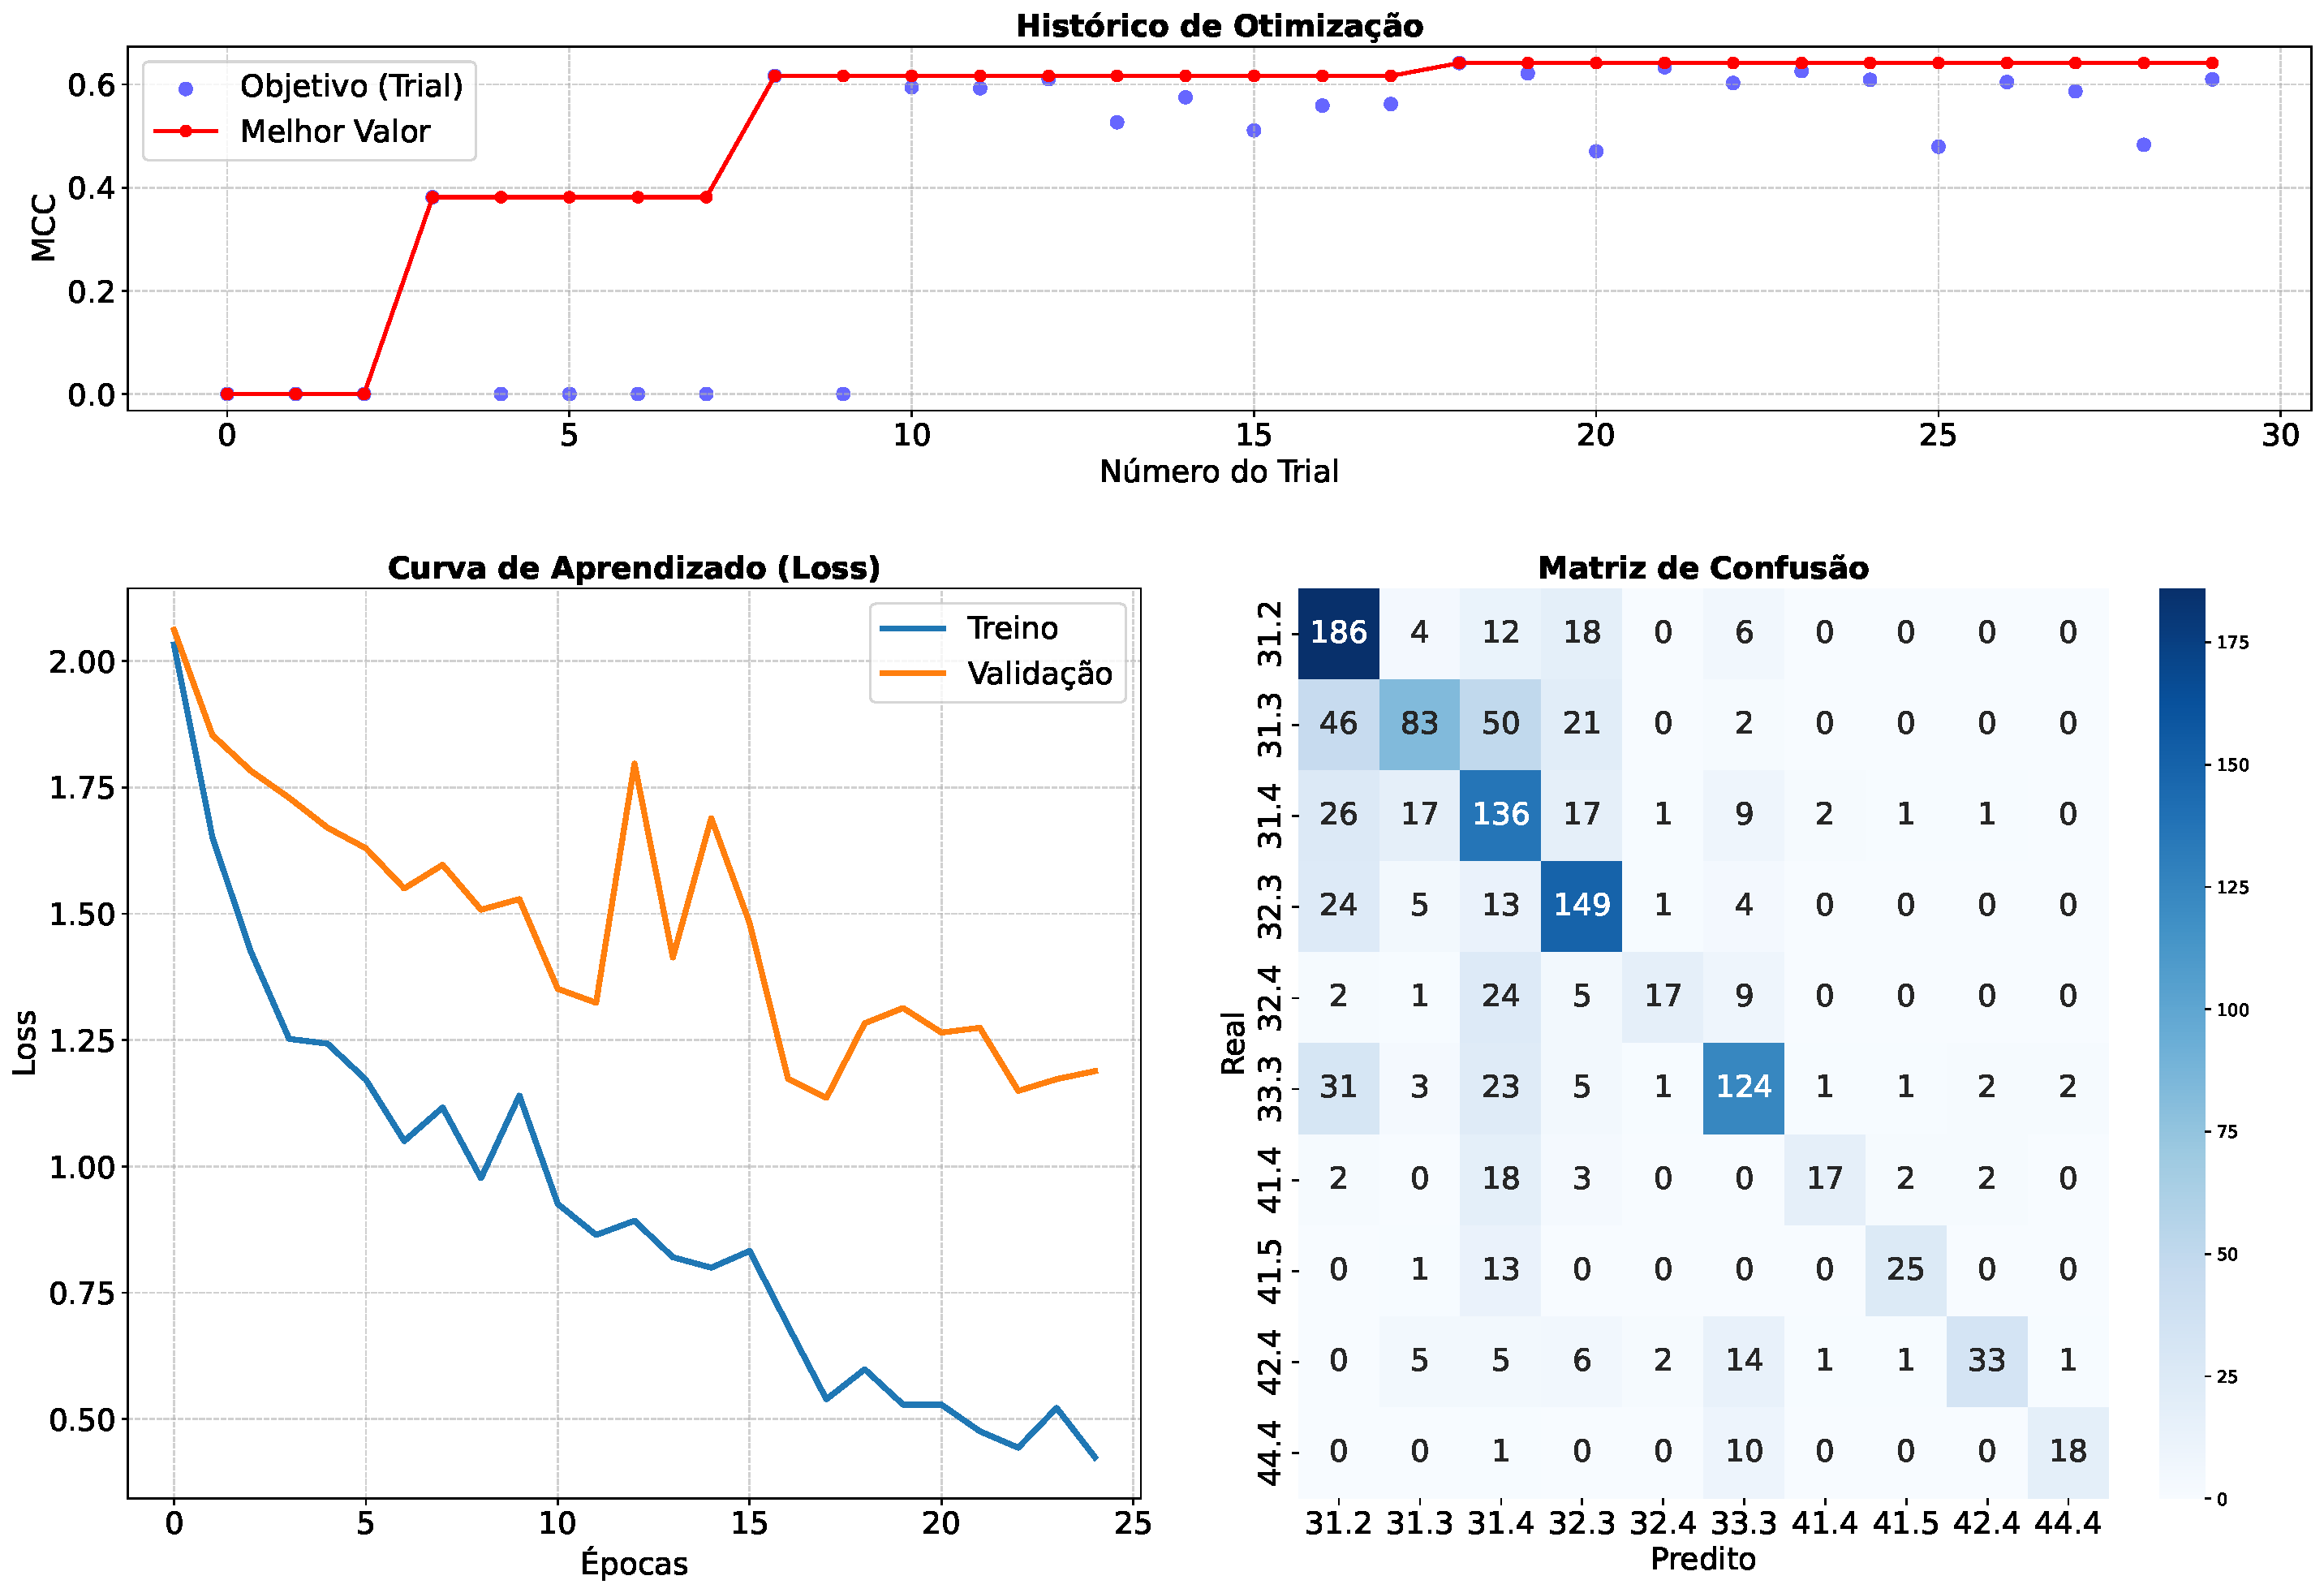
\includegraphics[width=0.85\textwidth]{tex/appendix/experiments/vgg_v1_AB_opt_aug/dashboard_consolidado.pdf}
        \caption{Histórico de Otimização, Curvas de Aprendizado e Matriz de Confusão - vgg\_v1\_AB\_opt\_aug}
    \end{figure}
\end{minipage}
\clearpage
